\documentclass[
  de, % or de
  inputenc=utf8,
  %aspectratio=169,
]{tuhhslides}

% use flat boxes
\setbeamertemplate{blocks}[flat]


% setup title, author and institute
\title[Reverse Engineering of a Jura Coffee Machine]{Reverse Engineering of a \\ Jura Coffee Machine}
\author[]{\speaker{Niklas Joachim Eberhard Kr\"uger}}
%%% as Student do not use any Institute tag or use the following
\institute{InstSchoolOfEEIT}
%%%
%%% as Staff you can use your Institute see tuhhlangnames.def
%\institute{InstTelematics}
%\institute{InstSmartPort}
%%%
\subject{Antrittsvortrag, Bachelorarbeit, Meyer}
\date{21.11.2018}

%%
\usepackage{listings}

% %% enable section page
% \AtBeginSection{%
%   \frame[plain,noframenumbering]{\sectionpage}
% }

\begin{document}

%% title page
\begin{frame}[plain,noframenumbering]
    \titlepage
\end{frame}

%% table of content
\begin{frame}
    \frametitle{\"Ubersicht}
    \tableofcontents
\end{frame}



\section{Aufbau}
% Jura
% Kabel
% Aduino
% PC
% (Fotos), Beschreibung und Aufgaben der Teile
\begin{frame}
  \begin{center}
    \begin{tikzpicture}
      \node (img1) {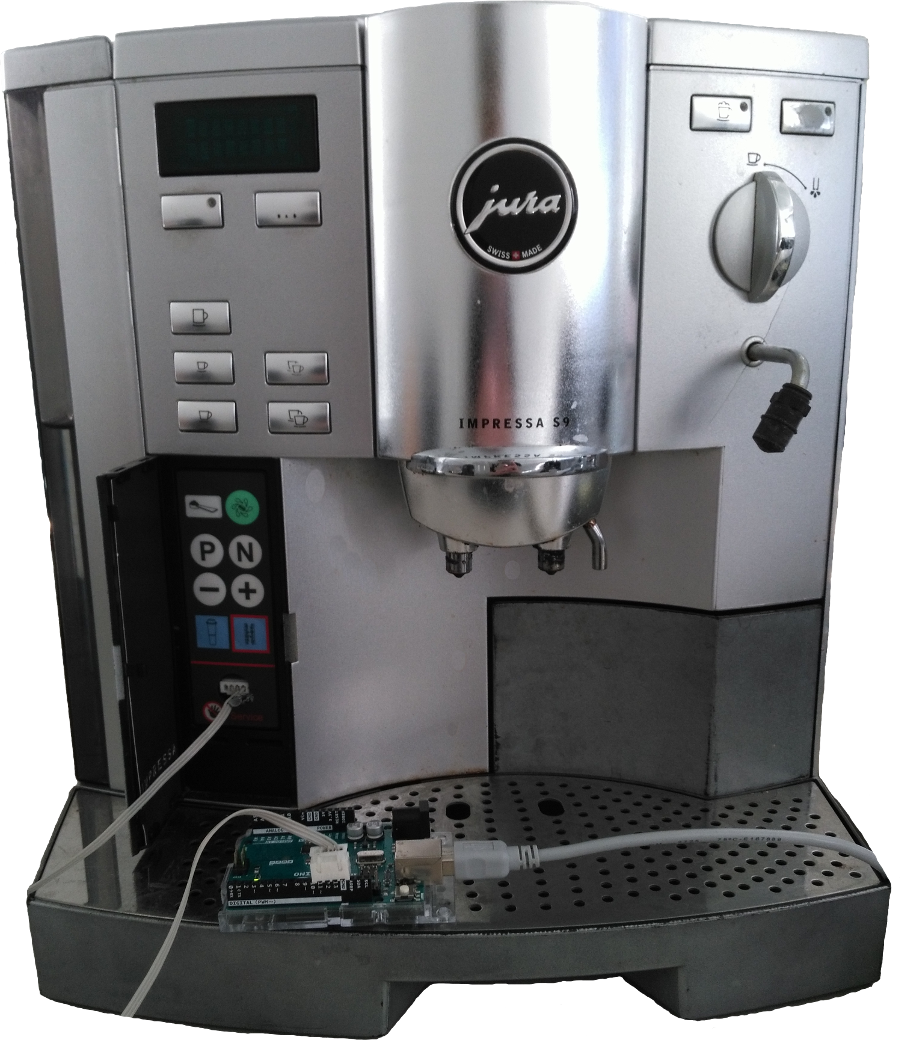
\includegraphics[scale=0.21]{Material/Jura-Impressa-S9-small.png}};
      \only<2>{
        \node (img2) at (img1.south west) [yshift=1.6cm,xshift=2cm] {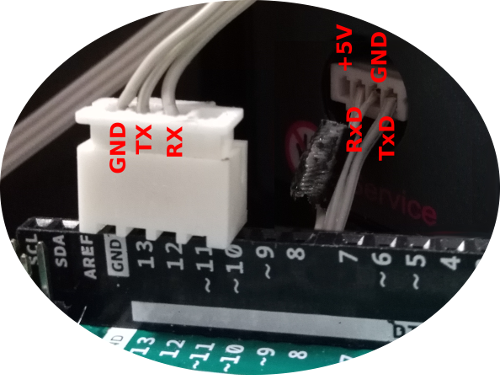
\includegraphics[scale=0.25]{Material/Jura-Arduino-Pins-beschriftet-small.png}};
      }
    \end{tikzpicture}
  \end{center}
\end{frame}

\begin{frame}{Verkabelung}
  \begin{itemize}
    \item Über eine serielle Schnittstelle kommunizieren Kaffee-Maschine und Arduino, sowie Arduino und PC
    \item Arduino kodiert die ASCI Befehle um in UART\footnote{Universal Asynchronous Receiver Transmitter}  Bytes, welche Kaffee-Maschine vesteht und vice versa
    \item Linux bindet den Arduino über \underline{/dev/ttyACM0} ein \\
          Die Baudrate liegt bei 9600
  \end{itemize}
\end{frame}

\begin{frame}{Kommandos}
	\begin{itemize}
    \item AN: Betriebszustand
    \item FA:<id> Bezugstaste
    \item FN:<id> Steuerungskomponente
    \item IC: Eingabe Status*
    \item PM: Play music, easter egg*
    \item RE:<address> Liest 2 Byte EEPROM Speicher
	  \item \alert<2>{RR:<address> Liest eine Zeile Ram}
	  \item \alert<2>{RT:<address> Liest eine Zeile EEPROM}
    \item TY: Maschinen Typ
    \item WE:<address>,<value> Schreibt 2 Byte in EEPROM
    \item ?M3 Aktiviere Inkassomudus
    \item ?M1 Deaktiviere Inkassomodus
    \item ?D<row><8 chars> Row-te Displayzeile
    \item ...
	\end{itemize}
	* ggf. nicht alles implementiert
\end{frame}



\section{Speicherschema}
\begin{frame}{EEPROM}
  \begin{figure}
    \begin{center}
      \hspace*{-1cm}
      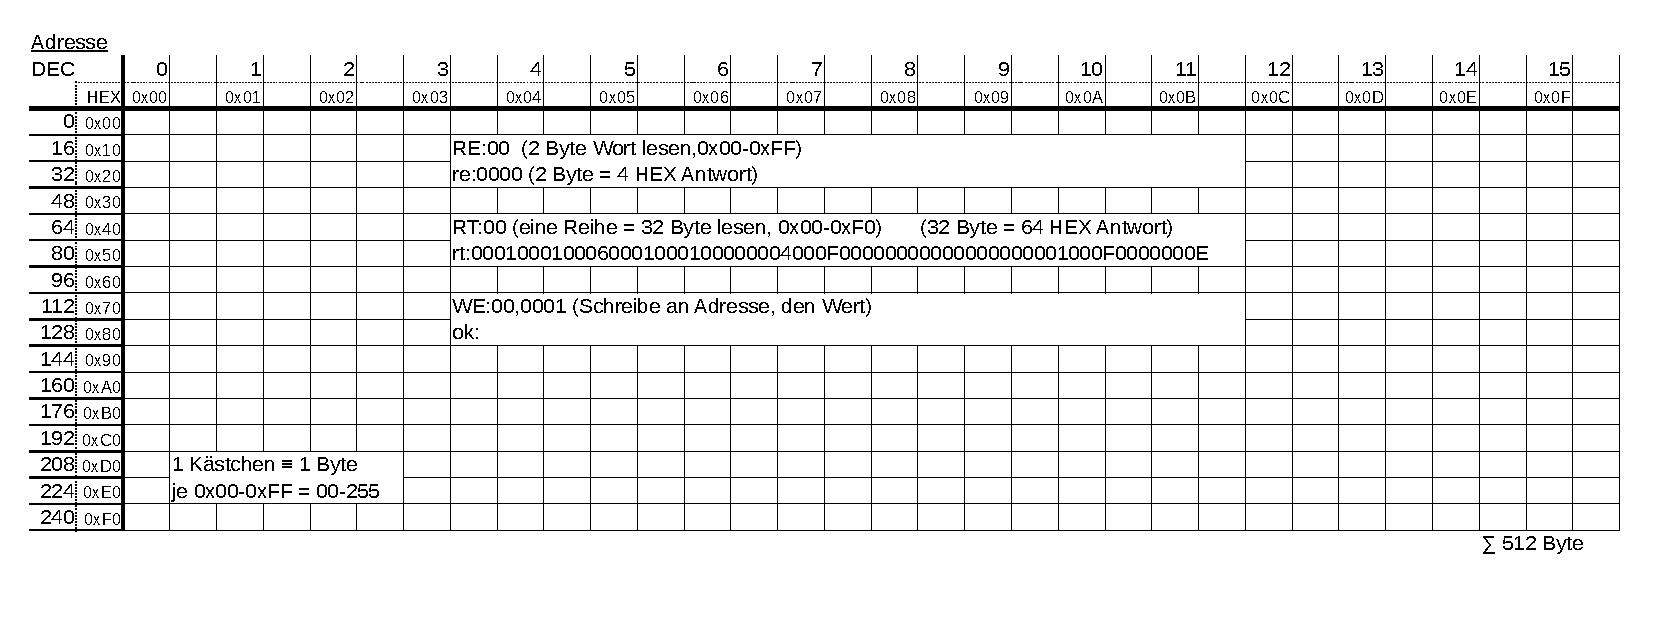
\includegraphics[scale=0.46]{Material/Speicher-Schema-Jura-EEPROM}
    \end{center}
  \end{figure}
\end{frame}

\begin{frame}{RAM}
  \begin{figure}
    \begin{center}
      \hspace*{-1cm}
      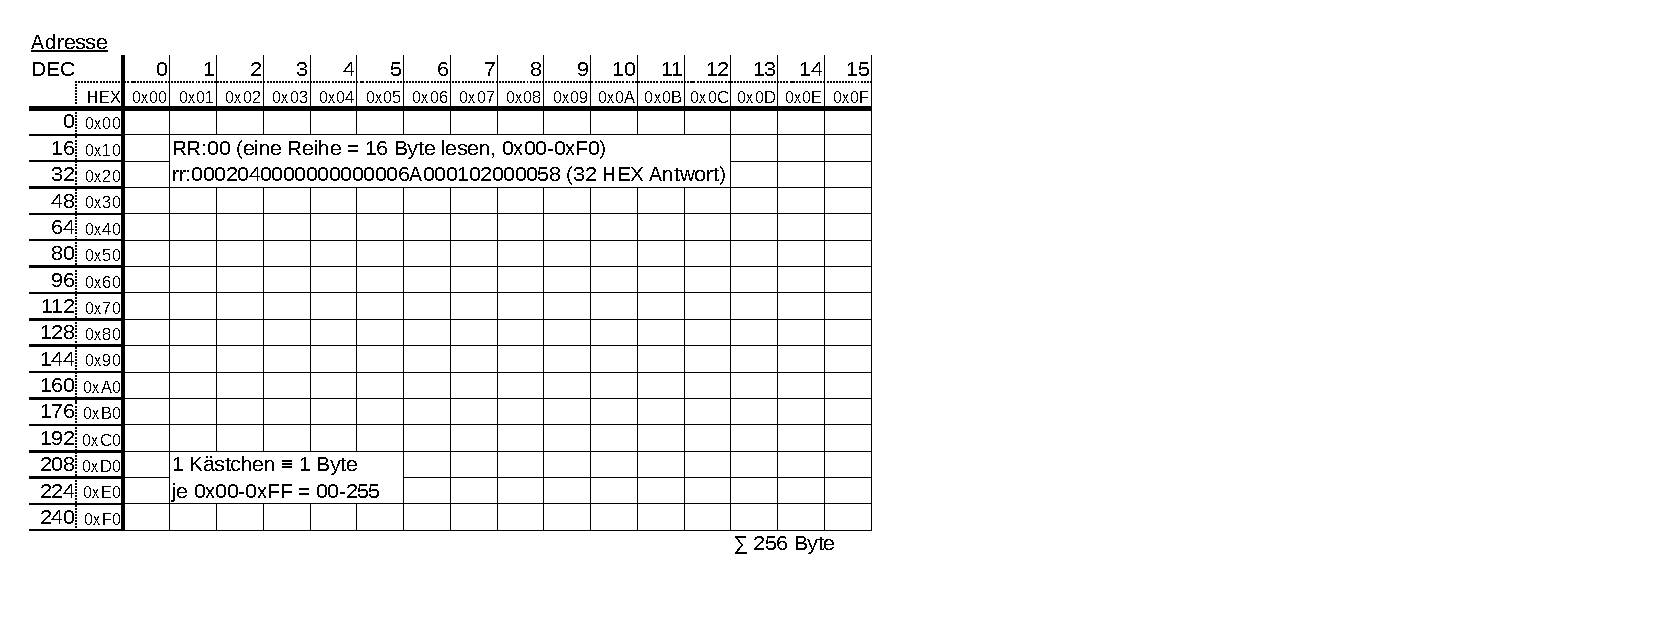
\includegraphics[scale=0.46]{Material/Speicher-Schema-Jura-Ram}
    \end{center}
  \end{figure}
\end{frame}



\section{Meine Aufgabe}
\begin{frame}{Aufgabenstellung / Thema}
	\begin{itemize}
		\item Reverse Engineering des Speichers
		\item Welches Wort / Byte / Bit speichert welche Information?
		\item Zugang zum Speicher:
		\begin{itemize}
		  \item direkt: Während des Betriebs schwierig
		  \item seriell: Über die vorhandene Schnittstelle, langsam
		\end{itemize}
	\end{itemize}
\end{frame}

\begin{frame}{Vorgehen}
	\begin{itemize}
		\item EEPROM und Ram über ein Skript auslesen
		\item Nach möglichst elementaren Veränderungen wiederholen
		\item Zustände und Speicherbereiche, sowie deren Bedeutung für die Kaffeemaschine ermitteln
		\item Ausbauen mithilfe weiterer Literatur
		\item Reverse Engineering im allg. hierzu in Relation setzen
		\item Ausblick: EEPROM gezielt (fern-)steuern
		\begin{itemize}
		  \item Per Knopfdruck wird der Kaffee nach eigenen Präferenzen zubereitet
		  \item Profile für Wasser-, Pulvermenge, Temperatur, ...
		\end{itemize}
	\end{itemize}
\end{frame}

\begin{frame}{Zeitplan}
  \begin{figure}
    \begin{center}
      \hspace*{-1cm}
      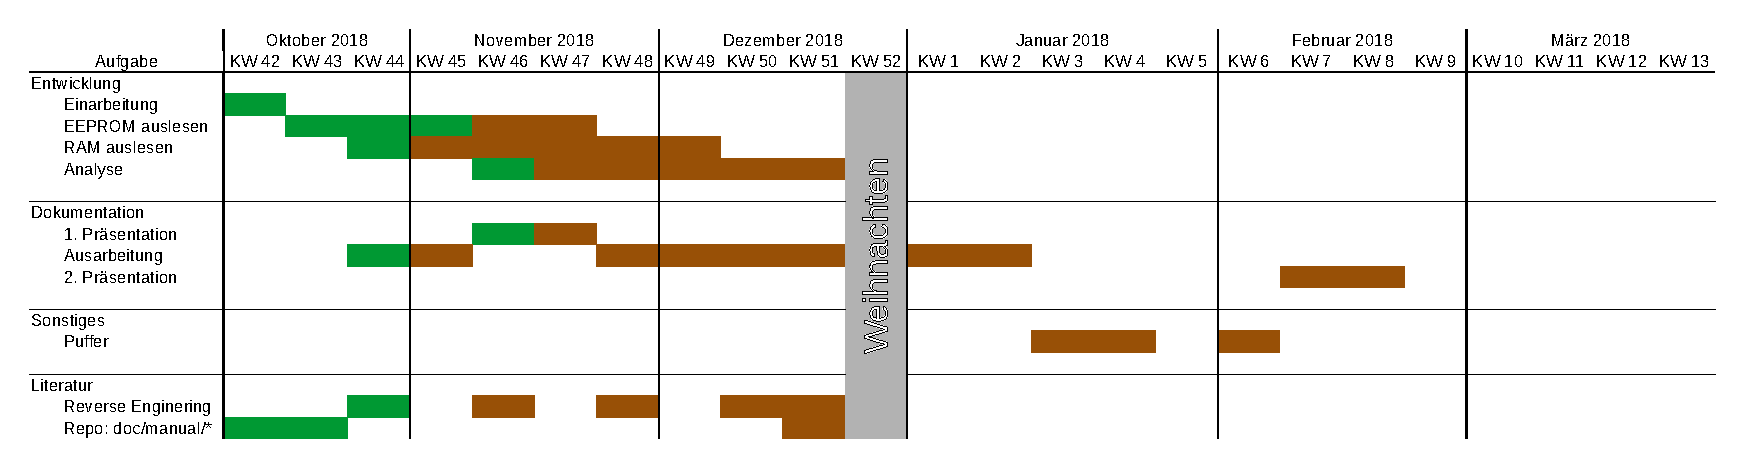
\includegraphics[scale=0.513]{Material/Zeitplan}
%       \caption{}
%       \label{fig:}
    \end{center}
  \end{figure}
\end{frame}



\backup

\begin{frame}
  \centering \LARGE
  Vielen Dank für die Aufmerksamkeit!
\end{frame}

\section*{Und los geht's...}

% \begin{frame}{Ergebnisse}
%   Folgen in Kürze
% \end{frame}



\end{document}
